%========================= CAPITULO 2 ==============================

\chapter{Revisão Bibliográfica} %\label{cap_exemplos}
%\thispagestyle{empty}
\section{Telefonia convencional}
\subsection{Funcionamento e organização da telefonia convencional}

Alexander Graham Bell, ao ligar para seu assistente em outra sala dizendo: “Senhor Watson, venha para cá. Quero falar com você”, concretizava a primeira transmissão, conversa telefônica em 10 de março de 1876, porém era apenas um simples fio que conectava os dois dispositivos, não havendo nenhum número para discagem, nem mesmo um som para indicar o funcionamento do aparelho, era basicamente uma ligação ponto a ponto do tipo half-duplex\footnote{Fluxo de dados unidirecional quando o envio e o recebimento de dados não são executados ao mesmo tempo} \cite{maxaltman2010}.

Mas o projeto evoluiu de uma única transmissão de sentido único de voz, onde apenas um usuário poderia falar, para uma transmissão bidirecional de voz, proporcionando aos usuários que ambos possam interagir na conversação telefônica. A voz era transmitida através de fios e era preciso um microfone de carbono, uma bateria, um eletroímã e uma diafragma de ferro. Ainda era preciso um meio físico entre as duas localidades que necessitavam se comunicar, e não havia o conceito de discagem \cite{eduardomaronasmonks2006}.

A figura \ref{Figura1}, ilustra a conexão física necessária através de cabos, onde era nescessário a conexão entre todos eles, fazendo assim o uso de sete cabos.
\begin{figure}[h]
	\centering
	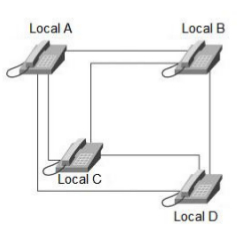
\includegraphics[width=6.0cm]{imagens/rebeBasicaQuatroTel.jpg}
	\caption{Conexão física entre quatro aparelhos telefônicos.}
    \label{Figura1}
    Fonte: \cite{davidson2008}
\end{figure}

Nos dias de hoje esse sistema seria impraticável, pois seria necessário conectar um fio telefônico a cada aparelho telefônico para o qual se desejasse efetuar uma ligação telefônica. Como exemplo da figura \ref{Figura2}, onde existisse apenas oito aparelhos telefônicos, seria necessário no meio físico vinte e oito cabos diferentes, e em cada aparelho sete conexões diferentes \cite{eduardomaronasmonks2006}.

\begin{figure}[h]
	\centering
	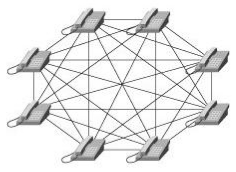
\includegraphics[width=6.0cm]{imagens/rebeBasicaOitoTel.jpg}
	\caption{Conexão física entre oito aparelhos telefônicos.}
    \label{Figura2}
    Fonte: \cite{davidson2008}
\end{figure}

O processo era custoso e havia pouca escalabilidade da estratégia e isto impossibilitou de imediato a expansão do sistema telefônico, mas com o passar do tempo houve a expansão com uso de comutadores (\textit{switches}), onde o sistema de telefonia na necessitava mais de uma ligação física direta entre todos os aparelhos telefônicos dos usuários \cite{thiagowinkler2007}.

Os comutadores realizam a conexão de um usuário através de um único cabo até o escritório central, e de início os comutadores eram pessoas, ou seja, um operador que perguntava qual destino o usuário gostariam se comunicar, e então o operador realizava a manualmente a conexão entre os dois trajetos de voz, a figura 3 exemplifica com fica um operador centralizado para comutar as chamadas entre quatro usuários \cite{eduardomaronasmonks2006}.

\begin{figure}[h]
	\centering
	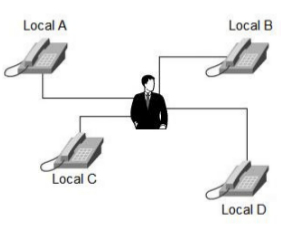
\includegraphics[width=7.0cm]{imagens/operadorCentralizado.jpg}
	\caption{Comutador Humano: Operador Centralizado.}
    \label{Figura3}
    Fonte: \cite{davidson2008}
\end{figure}

Os comutadores começaram a se tornarem automáticos, surgindo então o conceito de discagem para encontrar o destino das ligações, pois o números de ligações já estavam com grande volume, e conceito de comutadores manuais já estava impraticável. Os comutadores evoluirão de manuais, para eletromecânicos e consequentemente para eletrônicos com enorme capacidade de processamento. Através de técnicas de amplificação de sinal, bem como a automatização, digitalização e a escalabilidade necessária os serviços de telefonia permitiram a comunicação ao redor do mundo, com grande expansão. As duas formas de transmissão de voz na telefonia e a forma analógica e a forma digital. \cite{books/daglib/0018909}.

Por diversas décadas o sistema de telefonia permaneceu na estrutura analógica de transmissão, pois todo o som que se houve, inclusive o voz humana está no formato analógico. Em um sistema de telefonia de curto alcance, ou seja, de usuário próximo a central telefônica fazendo a ligação com outro usuário não era problema, porém com distancias cada vez maiores foi necessário a amplificação dos sinais de voz, mas devido a comunicação analógica os ruídos também são amplificados, ou seja, eram intensificados. Com relação aos PABX (\textit{Private Automatic Branch Exchange}), os ramais em sua maioria são analógicos com poucas exceções digitais dependendo dos recursos da central \cite{books/daglib/0018909}.

A solução empregada foi de regenerar os sinais em vez de amplificá-los, porém só é possível, por um processo de amostragem e quantização da amplitude dos sinais analógicos durante determinado período de tempo, ou seja,  por meio da sua digitalização, que transformam esses sinais em 0 (zeros) e 1 (uns) e posteriormente transmiti-los \cite{alexandrekeller2014}.

Para suprir a deficiência da transmissão analógica, surgiu então a transmissão digital, esta ainda permitiu que a voz fosse transferida em redes de pacotes. A digitalização da voz é realizada através de \textit{codecs} (codificadores/decodificadores) de voz, e sua transmissão e realizada por centrais telefônicas, ou seja, por \textit{backbone} das provedoras de serviços. Os comutadores realizam a conversão analógico/digital quando o sinal for em direção ao assinante. O PCM (\textit{Pulse Code Modelation}) é o \textit{codec} mais utilizado. Segundo \citeonline{gomeslemoscolcher1995}, as técnicas empregadas de amostragem são baseadas no teorema de Nyquist, onde o número de amostras deve ser duas vezes maior, do que a maior frequencia de sinal.

O processo de digitalização de voz usando PCM funciona da seguinte forma \cite{eduardomaronasmonks2006}:

\begin{figure}[h]
	\centering
	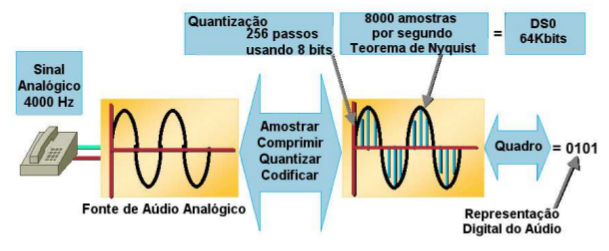
\includegraphics[width=16.0cm]{imagens/processoPCMdigital.jpg}
	\caption{Processo PCM de digitalização de voz.}
    \label{Figura4}
    Fonte: \cite{eduardomaronasmonks2006}
\end{figure}

\begin{itemize}
  \item As formas de ondas analógicas são passadas por um filtro de voz para eliminar qualquer freqüência acima de 4000 Hz. Estas freqüências são filtradas até 4000 Hz para limitar a quantidade de interferência entre linhas (crosstalk) na rede de voz.
  \item É feita a amostragem do sinal analógico na taxa de 8000 vezes por segundo.
  \item Após a amostragem, o sinal é convertido em um formato digital discreto. A amostra é representada por um código que indica a amplitude da forma de onda no instante da amostragem. O PCM utilizado em telefonia usa 8 bits em cada amostra.
\end{itemize}
	
O PCM utiliza largura de banda nas chamadas de 64 Kbps também conhecido como DS-0, sendo que utiliza um código de de 8 bits registrado 8000 vezes por segundo para a codificação dos sinais de áudio, é o equivalente a um circuito de 64 Kbps (8 bits x 8000s) \cite{alexandrekeller2014}.

Existe duas variações de codificações do PCM, o padrão de codificação norte americano e japonês, que é G.711u também conhecido como m-law, e ainda o padrão de codificação europeu e de outros países inclusive o Brasil que é o G.711a também conhecido como a-law, possuem minímas diferenças, onde o m-law tem uma pequena vantagem sobre à performance na sinalização de ruídos de baixo nível \cite{gomeslemoscolcher1995}.

\subsection{Infra-estrutura da PSTN}
O atual sistema de telefonia, também chamado de PSTN (\textit{Public Switch Telephone Network}), foi planejado para acomodar uma única aplicação, ou seja, a voz não comprimida. Estas redes foram construídas para entregar 99,9994$ \% $ das chamadas, com baixa latência, e roteamento de chamadas altamente escalável através da infra-estrutura SS7 (\textit{Signaling System 7}, e serviços de voz de valor agregado como mensagem de voz e identificador de chamadas.

A infraestrutura inicial de telefonia começa com os pares de fios conectados ao terminal telefônico, chamado local loop, estes pares de fios são conectados a uma central telefônica, seja ela uma central particular como um PABX ou um provedor de serviços de telefonia. O tronco (\textit{trunk}) é a comunicação entre comutadores centrais ou entre PABXs. \cite{eduardotude2014}.

\subsubsection{Tipos de sinalização e estabelecimento de circuitos}
A sinalização é realizada em dois sentidos, usuário/rede telefônica e rede telefônica/rede telefônica. A primeira situação é a forma de como usuário final se comunica com a rede telefônica, geralmente através de um um terminal analógico. O DTMF (\textit{Dual Tone Multi-Frequency}) é o método mais comum, e possibilita através da variação da frequência representar dígitos e comandos no terminal telefônico, sua transmissão ocorre no mesmo caminho da voz, conhecido como sinalização inband \cite{thiagowinkler2007}.

Existem protocolos de sinalização inband e outband. Os protocolos inband entre centrais foram abolidos nos anos 70, por limitações técnicas e por serem susceptíveis a fraudes. O protocolo outband possui um caminho independente da voz, como o protocolo SS7 (\textit{Signaling System 7}), este protocolo  reserva um canal de 64kbits para controle das chamadas e através de pacotes controla as conexões na central e entre centrais, permite ainda funções como identificação do telefone chamador e diminuição no tempo de complemento de chamadas, atualmente e protocolo padrão \cite{eduardomaronasmonks2006}.

As especificações dos sinais elétricos indicam se o circuito e circuito do tipo E1 ou T1, ou seja, a rede telefônica poder ser vista como uma malha de cabos e sinais elétricos, onde a especificações das variações dos sinais elétricos indica os eventos e ocorrências de cada circuito. Tanto no Estados Unidos como no Japão utilizam-se circuitos DS-0 de 24 grupos, os chamados T1, que fazem uso do codec m-law e ocupam 1544 Mbps, 24 canais de 64 Kbps, mais 8 Kpbs utilizados na sinalização dos frames de dados. Já na Europa e nos demais países utiliza DS-0 de 32 grupos, os chamados de E1, utilizando o codec a-law, sendo 30 canais de 64 Kbps para trafegar voz, 1 canal para sinalização e 1 para sincronia do link de comunicação, totalizando 2048 Mbps \cite{alexandrekeller2014}.

Os circuitos E1 que utilizam TDM (\textit{Time-Division Multiplexing}), são constituídos de canais fixos de voz, sinalização e sincronia, ou seja, o canal zero é sempre o canal de sincronia, o canal dezesseis e sempre o canal de sinalização, e são conhecidos como canais D (delta), e os demais canais B (Bearer), onde definitivamente trafega o áudio das chamadas, é exemplifica na figura \ref{Figura5} \cite{andersonramires2005}.

\begin{figure}[h]
	\centering
	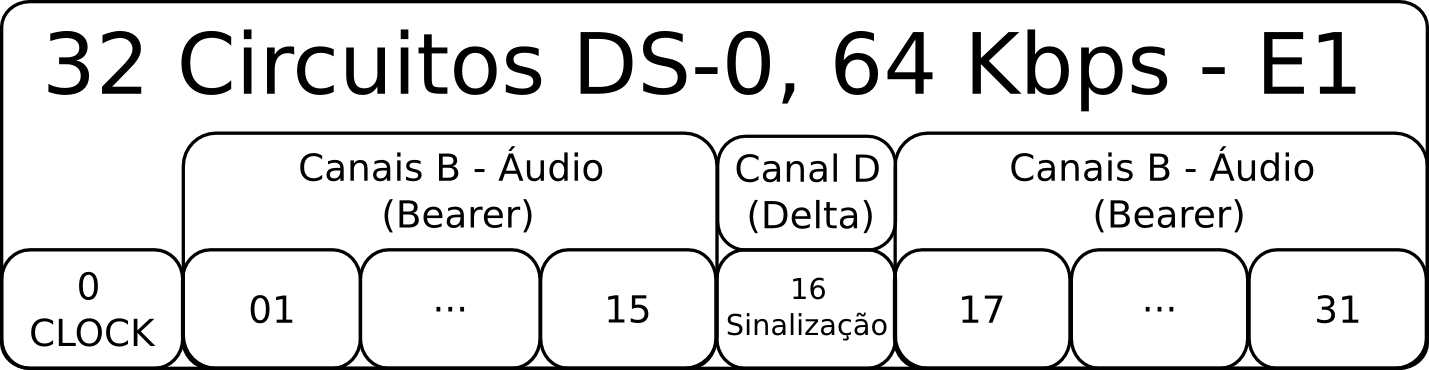
\includegraphics[width=15.0cm]{imagens/LinkE1.png}
	\caption{Diagrama de um circuito E1.}
    \label{Figura5}
    Fonte: \cite{alexandrekeller2014}
\end{figure}

\subsubsection{Estabelecimento de um circuito, ou chamada telefônica}

Não é apenas áudio que trafega durante uma chamada telefônica, ocorre uma série de trocas de sinais entre o originador da chamada e recebedor, onde a correta transmissão e a identificação desses sinais influenciam diretamente no correto estabelecimento e encerramento da chamada, pois um usuário A deseja se conectar a um usuário B, o usuário a retira do gancho o fone (\textit{off-hook}), e logo o equipamento a qual o telefone esta conectado emite um um sinal sonoro, ou seja, tom de discagem (\textit{dial tone}), isto avisa ao usuário que já pode digitar os dígitos referentes ao número de telefone do usuário B, o envio destes digitos até a operadora é realizado por DTMF (\textit{Dual-Tone Multri Frequency}), que a representação sonoro dos números 0 à 9 mais os sinais \# (\textit{sustenido}) e $ \ast $ (\textit{asterisco}) \cite{alexandrekeller2014}.

Cada país possui tons específicos de DTMF, e a operadora a identificar o termino dos envios dos dígitos, emiti um sinal de chamando (\textit{ringing}) para o usuário A, e ao usuário B atender, emite a operadora um sinal de (\textit{off-hook}), então o circuito é fechado, e a comunicação é estabelecida. A partir deste momento o som produzido pelo participantes da chamada é transmitido até que um dos usuários termine a conexão, colocando de volta o fone no guancho (\textit{on-hook}), gerando um sinal de desligamento (\textit{hangup}) para operadora, liberando assim o circuito que havia sido gerado \cite{eduardotude2014}.

Mas liberação desse circuito depende do lado de quem finalize a chamada, conforme normas brasileiras, se originador da chamada é o usuário A, os custos da chamada pertence a ele, então se ele finalizar a chamada, ela será finalizada de imediato, caso seja o usuário B, recebedor da chamada, a chamada continuara ativa por 90 segundos, pois que tem o direito de encerrar o circuito e só originador da chamada, porém se a chamada originar do usuário A, mas com cobrança direcionado ao usuário B, também conhecidas como “ligações a cobrar” o direito da desconexão passa para o usuário B \cite{andersonramires2005}.

O DTMF é amplamente utilizado em circuitos analógicos, mas existem outros dois digitais amplamente utilizados, que utilizam a sinalização CAS (\textit{Channel Associated Signalling}), sendo eles o MFC e o R2-Digital, ainda há a RDSI (\textit{Rede Digital de Serviços Integrada}), ou no inglês ISDN (\textit{Integrated Service Digital Network}), que utiliza a sinalização CCS (\textit{Commom Channel Signalling}) \cite{alexandrekeller2014}.

\subsubsubsection{Sinalização multi-frequency}
A sinalização MF (\textit{multi-frequency}) ou multifrequencial, utiliza de tons para permitir a troca de sinalização envolvida para o estabelecimento de uma chamada, já a sinalização MFC/R2-Digital, utiliza o MFC (\textit{Multi-Frequency Code}), pois a sinalização entre dois pontos depende de uma sequencia preestabelecida. Getalmente essa troca de sinalização ocorre da seguinte forma: \cite{davidson2008}

\begin{itemize}
  \item A envia um sinal multifrequencial e o mantém até que B o receba e confirme.
  \item O usuário B confirma o recebimento com outro sinal multifrequencial, essa confirmação também significa uma solicitação para A, e B mantém o sinal multifrequencial durante o processo.
  \item A percebe que B confirmou o recebimento do sinal multifrequencial e retira o sinal multifrequencial que o enviou, assim dependendo de que B solicitar A fica pronto para o envio de um novo sinal multifrequencial.
  \item B percebe que A retirou o sinal multifrequencial, e também retina seu sinal multifrequencial, e B fica apto a receber uma nova solicitação de A. O ciclo repete até o termino da troca de sinalizações entre os terminais de A e B envolvidos na chamada.
\end{itemize}

\subsubsubsection{Sinalização R2-Digital}

O padrão brasileiro de sinalização para links digitais de telefonia no padrão E1 é o R2-Digital comumente conhecido, por utilizar do CAS (\textit{Channel Associated Singalling}), ou simplesmente sinalização associada ao canal, acaba se tornando lento e inflexível. O CAS possui três grupos de sinais: \cite{thiagowinkler2007}

\begin{itemize}
  \item \textbf{Sinais de supervisão}, representam os eventos que ocorrem durante uma chamada e geralmente são específicos para cada variação do CAS de cada região ou país. São também chamados de sinais de linha (\textit{line signals}), e incluem requisição do canal (\textit{seizure}), wink e answer (\textit{atendimento}). No Brasil utilizamos  também o termo “sinalização de linha” para esses sinais, que estão associados ao canal dezesseis e representam os sinais de R2.
  \item \textbf{Sinais de endereçamento}, é o numero de destino, ou seja, os números enviados, são específicos para as variações do CAS implementadas em determinada região, utilizam como base a sinalização multifrequencial. Os tons multifrequenciais são utilizados para transmitir o ANI (\textit{Automatic Idendification Number}), conhecido de forma vulgar como DNIS (\textit{Dialed Number Identification Service}), ou simplesmente \textit{Caller ID}, que não verdade significa que são enviados o número de destino e categoria do originador da chamada. Esses sinais são conhecidos como sinalização de registro no Brasil, pois utiliza sinal multifrequencial através do canal D (\textit{delta}) para envio da sinalização de registro, onde corresponde ao circuito que será utilizado após a chamada ser completada, assim podemos dizer que a sinalização é associada ao canal, ou seja, ao CAS.
  \item \textbf{Tons de anúncios}, são os tons de ringing (\textit{chamando}), ocupado (\textit{busy}), ou mesmo anúncios de “\textit{o número chamado não existe}.
\end{itemize}

A sinalização MFC/R2-Digital trata de forma única e exclusivamente de sinais de áudio, ou seja, tons para identificação da troca sinalização, onde o sinal multifrequencial e enviado dentro do próprio canal de áudio e os sinais de supervisão R2 da chamada dentro do canal dezesseis, específico para essa finalidade. E a conversão dos sons para o meio digital exige grande poder de processamento \cite{davidson2008}.

\subsubsubsection{Sinalização ISDN}
O RDSI ou ISDN, foi concebido em meados dos anos 1980, é o modelo de sinalização para circuitos de telefonia TDM, considera-se como a evolução natural do MFC/R2, pois além de trafegar áudio, ele trafega também todos os tipos de informação, como mensagens de texto, e até mesmo video. Utiliza um canal único para a sinalização da chamada, o CCS (\textit{Commom Chanel Signalling}), mais precisamente o canal dezesseis do circuito, através de pacotes de dados no formato Q.931. O Q.931 controla as requisições e respostas às mensagens de setup da chamada, o reconhecimento do setup, progresso da chamada, mensagens de alerta, desconexão (desligamento) e de informações \cite{alexandrekeller2014}.

O Brasil adotou o EUROISDN como padrão de configuração para ISDN, porém existe outros modelos como o 4ESS, 5ESS, NI1 e Q.Sig. Um circuito E1 ISDN é conhecido como PRI (\textit{Primary Rate Interface}), ou ainda, 30B+D, em referencia aos trinta canais de dados (B – \textit{Bearer}), e um canal de sinalização (D – \textit{Data}).

O ISDN é extremamente rápido e flexível comparado ao MFC/R2, e é semelhante o protocolo TCP/IP usando pacotes de dados para transportar as informações. Mas ainda existem localidades no Brasil onde as centrais telefônicas são antigas e não houve investimento em atualização tecnológicas por parte das operadoras de telefonia, principalmente nas regiões Norte, Nordeste e Centro-Oeste e nestas localidades só tem disponível a sinalização MFC/R2 \cite{eduardotude2014}.

\subsubsection{Termos referentes a Links E1}
Alguns termos utilizados quando nos referimos a links E1, seja com sinalização MFC/R2 ou com ISDN: \cite{alexandrekeller2014}

\begin{itemize}
  \item \textbf{Alinhamento}, o link E1 deve sempre alinhando, ou seja, o canal de comunicação 1 (um) de lado do circuito deve estar alinhado com o canal 1 (um) do outro lado do circuito. O alinhamento e estabelecido pelo lado do circuito configurado como originado do clock, ou seja, é o lado que vai estabelecer o início do alinhamento dos 30 canais de comunicação do link E1.
  \item \textbf{Escorregamento}, é a perda do alinhamento entre os canais, em decorrência da perda de sincronia do clock, onde por exemplo o canal 10 (dez) de um lado não esta mais alinhado com o canal 10 do outro lado do circuito.
  \item \textbf{TAPS}, é o cancelamento do eco, ou mesmo supressores de eco, onde após realizarem a identificação e o treinamento (echotraining) do nível do eco dentro da ligação, aplicam os filtros ao áudio da chamada dependendo do valor do TAPS, como 32 TAPS (4 ms), 64 TAPS (8 ms), 128 TAPS (16 ms ), 256 TAPS (32 ms) e 512 TAPS (64 ms).
\end{itemize}